\documentclass[11pt,aspectratio=169]{beamer}
\usepackage[T1]{fontenc}
\usepackage{lmodern}
\usepackage{booktabs,array,tabularx}
\usepackage{tikz}
\usetikzlibrary{arrows.meta,positioning,fit,backgrounds,calc}
\usepackage{listings}
\definecolor{Navy}{HTML}{162B43}
\definecolor{Teal}{HTML}{007E80}
\definecolor{Amber}{HTML}{986400}
\definecolor{Rust}{HTML}{AA3C35}
\definecolor{Ink}{HTML}{243749}
\definecolor{Muted}{HTML}{586B7C}
\definecolor{Pale}{HTML}{EDF4F7}
\definecolor{Mint}{HTML}{E8F4F1}
\definecolor{Sand}{HTML}{FFF3D9}
\setbeamercolor{normal text}{fg=Ink,bg=white}
\setbeamercolor{structure}{fg=Teal}
\setbeamercolor{frametitle}{fg=Navy}
\setbeamercolor{title}{fg=Navy}
\setbeamercolor{subtitle}{fg=Muted}
\setbeamercolor{block title}{fg=white,bg=Navy}
\setbeamercolor{block body}{fg=Ink,bg=Pale}
\setbeamercolor{block title alerted}{fg=white,bg=Amber}
\setbeamercolor{block body alerted}{fg=Ink,bg=Sand}
\setbeamerfont{title}{size=\LARGE,series=\bfseries}
\setbeamerfont{frametitle}{size=\Large,series=\bfseries}
\setbeamerfont{subtitle}{size=\large}
\setbeamerfont{block title}{size=\normalsize,series=\bfseries}
\setbeamersize{text margin left=8mm,text margin right=8mm}
\setbeamertemplate{navigation symbols}{}
\setbeamertemplate{itemize item}{\color{Teal}\small$\blacktriangleright$}
\setbeamertemplate{itemize subitem}{\color{Teal}\scriptsize$\bullet$}
\setbeamertemplate{frametitle}{\par\vspace{3mm}\insertframetitle\par\par\vspace{1.5mm}\textcolor{Teal}{\rule{\textwidth}{0.6pt}}}
\setbeamertemplate{footline}{%
 \hbox{\begin{beamercolorbox}[wd=.81\paperwidth,ht=3.3ex,dp=1.2ex,leftskip=8mm]{normal text}
 \color{Muted}\tiny CONNECTION MANAGEMENT\quad /\quad 17 NOV 2026\quad /\quad THROUGH INCREMENT 100
 \end{beamercolorbox}%
 \begin{beamercolorbox}[wd=.19\paperwidth,ht=3.3ex,dp=1.2ex,rightskip=8mm plus 1fil]{normal text}
 \hfill\color{Muted}\tiny\insertframenumber\ /\ \inserttotalframenumber
 \end{beamercolorbox}}}
\newcommand{\evidence}[1]{\vfill{\fontsize{7}{8}\selectfont\color{Muted}Evidence: #1\par}}
\newcommand{\status}[2]{\textcolor{#1}{\textbf{#2}}}
\newcommand{\code}[1]{\texttt{\small #1}}
\pdfstringdefDisableCommands{\def\translate#1{#1}}
\newcolumntype{P}[1]{>{\raggedright\arraybackslash}p{#1}}
\newcolumntype{Y}{>{\raggedright\arraybackslash}X}
\tikzset{
 box/.style={draw=Teal!50,fill=Pale,rounded corners=2pt,align=center,inner sep=5pt,font=\small},
 pending/.style={box,draw=Amber,dashed,fill=Sand},
 arrow/.style={-{Latex[length=2mm]},thick,draw=Teal},
 label/.style={font=\scriptsize,text=Muted,align=center}
}
\lstset{basicstyle=\ttfamily\scriptsize,breaklines=true,columns=fullflexible,keepspaces=true,showstringspaces=false,backgroundcolor=\color{Pale},frame=none,xleftmargin=2mm,xrightmargin=2mm}
\title{Source-aligned\ connection management}
\subtitle{Shutdown, design exploration and scoped gate acceptance}
\author{Project progress briefing}
\date{17 November 2026}

\begin{document}

\begin{frame}[plain]
\par\vspace{5mm}
{\color{Teal}\small AGDA / CARDANO NETWORK / CONNECTION MANAGEMENT}\par\vspace{6mm}
{\usebeamerfont{title}\color{Navy}Source-aligned\par connection management}\par\vspace{4mm}
{\large Shutdown certificates, source findings and a correct design}\par\vspace{6mm}
\begin{beamercolorbox}[sep=3mm,wd=\textwidth]{block body}
\textbf{Branch review through Supervision increment 100}\par
\small Scoped G0--G5 acceptance, endpoint quiescence in Agda, and a pinned Haskell prototype.
\end{beamercolorbox}
\vfill\small 17 November 2026\hfill Standalone \texttt{ConnectionManagement/} model
\end{frame}

\begin{frame}{Two objectives now have equal standing}
\begin{block}{Find source problems}
Execute CM, IG, OG and Server together to expose connection-lifetime, cleanup and supervision faults.
\end{block}\begin{block}{Establish a correct design}
State intended guarantees, prove reachable-state properties and compare proposed changes with the same source-derived rule families.
\end{block}\small The combined subsystem remains the subject. A successful finite witness and a universal model invariant answer different questions.
\evidence{DESIGN, section 1; DesignContract, sections 1--2.}
\end{frame}

\begin{frame}{Findings and design status}
\small\renewcommand{\arraystretch}{1.2}
\begin{tabularx}{\textwidth}{@{}P{27mm}Y@{}}
\toprule
Topic & 17 November review \\ \midrule
Source findings & The seven classifications still stand. A pristine full-Server control adds evidence that shutdown did not wait for a self-purged handler. \\[2mm]
Agda proof & SI5 certifies the collected-handler wait. The registry variant certifies historical results and worker joins at reached endpoints. \\[2mm]
Haskell prototype & Increment 100 tests both joins and the sweep at the pin. Ordering differs from Agda, and progress failures remain. \\[2mm]
Gates & G0--G5 are met within their model, contract and finite exploration scopes. \\[2mm]
\bottomrule
\end{tabularx}
\evidence{CM\_Summary, sections 3--5. November architecture review, section 11. Supervision increment 100.}
\end{frame}

\begin{frame}{The source baseline advanced on 9 November}
\small\renewcommand{\arraystretch}{1.2}
\begin{tabularx}{\textwidth}{@{}P{28mm}Y@{}}
\toprule
Authority & Current role \\ \midrule
Network \code{2f1c154f2486} & Promoted implementation baseline after the M0--M6 migration. \\[2mm]
Consensus \code{2e44d98a8431} & Pins that network revision and supplies the reviewed application bundle. \\[2mm]
Earlier results & Retain their original network \code{96ee6e0} / consensus \code{585a861} pins. \\[2mm]
Branch review & Model \code{687463c} on \code{kangfeng/connection\_manager}. Increment 100 is a separate patch against the promoted network pin. \\[2mm]
\bottomrule
\end{tabularx}
\evidence{SourceLedger. SourceReplay M6 and increment 100. November architecture review, section 11.}
\end{frame}

\begin{frame}{Three kinds of evidence stay separate}
\begin{itemize}\setlength\itemsep{2.5mm}
\item \textbf{Model proof:} all executions satisfying a theorem\textquotesingle s exact initializer and premises.
\item \textbf{Source fidelity:} a reviewed mapping to named operations, branches and dependency contracts at the pin.
\item \textbf{Replay:} selected implementation operations under recorded synthetic inputs, schedules and controls.
\end{itemize}\begin{alertblock}{Gate acceptance has a scope}
The finite LocalLifecycle profile, full raw semantic rendering and declared search alphabets each have different acceptance boundaries.
\end{alertblock}
\evidence{GateAudit introduction and G0--G5; DESIGN, sections 1 and 9; SourceReplay/README.}
\end{frame}

\begin{frame}{Shutdown coverage grew before the SI5 proof}
\small\renewcommand{\arraystretch}{1.2}
\begin{tabularx}{\textwidth}{@{}P{28mm}Y@{}}
\toprule
Route & Progress since increment 63 \\ \midrule
Outbound mux & Actual CM receipt derives collection and initialized handler resources. \\[2mm]
TIME\_WAIT & Elapsed/interrupted cleanup routes and release-caller delivery preserve captured identity and the protected finally. \\[2mm]
External interrupt & Accept loops close before action cancellation; the peer side remains live until its own unwind. \\[2mm]
IG / accept failure & IG-first deactivation/flush/rethrow and accept-first listener cleanup reach the shared teardown chain. \\[2mm]
\bottomrule
\end{tabularx}
\evidence{Supervision increments 64--70; ServerPeersMuxReceipt, ServerPeersTimeWaitReceipt, ServerPeersReleaseTimeWait. Selected one-listener paths.}
\end{frame}

\begin{frame}{SI5a derives the outer shutdown certificate}
\begin{block}{Premise}
An initialized outer execution reaches \texttt{finished} relays.
\end{block}\begin{itemize}\setlength\itemsep{2.5mm}
\item Server is at \texttt{serverReturned}.
\item Governor and PSA monitor pools are closed, with their coordinator finished.
\item Snapshot jobs have Async results and all four inner scopes are joined.
\item Relays are absent as configured, or their thread is joined.
\end{itemize}\small This derives the component facts from one composed history. It does not assume a supplied whole-system completion flag.
\evidence{Supervision increment 71; Properties/ServerShutdownComplete, Protocols.complete. Endpoint safety, with no eventuality or fairness theorem.}
\end{frame}

\begin{frame}{SI5b certifies CM closure and the actual wait}
\begin{itemize}\setlength\itemsep{2.5mm}
\item The CM coordinator is \texttt{closed}, with no unread captured snapshot entries.
\item The closing \texttt{finishClose} is an actual wrapper transition.
\item Its physical wait reads that wrapper\textquotesingle s handler-result table and finds every collected result available.
\end{itemize}\begin{alertblock}{Snapshot scope}
This certifies collected handlers at the wait. Raw admission workers and handlers outside or after the snapshot remain excluded. It does not assert that every historical handler ended.
\end{alertblock}
\evidence{Supervision increment 72; Properties/ServerShutdownCoordinator, CMClosed. One listener and initialized outer histories reaching finished relays.}
\end{frame}

\begin{frame}{Residue c1: the IG leaves no pending CM call}
\begin{block}{At finished relays}
The IG is exited and deactivated. Both its pending inbound-release call and its pending remote-state call are absent.
\end{block}\begin{itemize}\setlength\itemsep{2.5mm}
\item Quietness is preserved through machine, peer, Server and runtime steps.
\item The proof uses actual call writers and the IG join boundary.
\item Raw admission workers are a separate lifetime and remain outside c1.
\end{itemize}
\evidence{Supervision increment 74; Properties/IGPendingQuiet, Protocols.ig-quiet. Same initialized outer shutdown profile as SI5.}
\end{frame}

\begin{frame}{Residue c2 exposed foreign callers in the model}
\begin{block}{Original statement fails}
An externally owned acquire frame can survive peer shutdown and finished relays while SI5 and c1 both hold.
\end{block}\begin{block}{Restated source-model theorem}
Every residual acquire/release frame belongs to a worker owned by neither a governor job nor a peer monitor.
\end{block}\small Production CM calls come from peer-state actions. An arbitrary retained CM-handle caller is a model over-approximation, whose stack the CM does not own.
\evidence{Supervision increments 75--76; Negative/ForeignCallerResidue; Properties/ForeignFrames. Explicit O.initial premise.}
\end{frame}

\begin{frame}{Late admission can escape the CM snapshot}
\centering
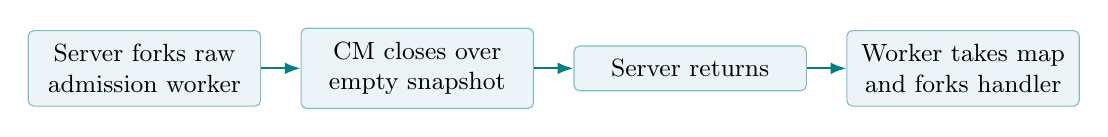
\begin{tikzpicture}[node distance=6mm and 5mm]
\node[box,text width=26mm] (fork) {Server forks raw admission worker};
\node[box,text width=26mm,right=of fork] (cm) {CM closes over empty snapshot};
\node[box,text width=26mm,right=of cm] (ret) {Server returns};
\node[box,text width=26mm,right=of ret] (late) {Worker takes map and forks handler};
\draw[arrow](fork)--(cm);\draw[arrow](cm)--(ret);\draw[arrow](ret)--(late);
\end{tikzpicture}
\par\vspace{5mm}
\begin{itemize}\setlength\itemsep{2.5mm}
\item The initialized Server-layer witness executes these steps through the real dispatcher.
\item The source drops the admission Async handle and has no include shutdown guard.
\item The model run is at the admission layer, without a new fully composed late-admission proof.
\end{itemize}
\evidence{Supervision increment 73; Negative/ServerLateAdmission; Server.hs:239--254 and Core.hs:524--550 at the promoted pin.}
\end{frame}

\begin{frame}{Late-admission replay leaves one link unconfirmed}
\small\renewcommand{\arraystretch}{1.2}
\begin{tabularx}{\textwidth}{@{}P{28mm}Y@{}}
\toprule
Observation & What the replay establishes \\ \midrule
Server IOSimPOR & Server and CM return while their own accepted worker has not started its include. \\[2mm]
Direct CM API & A retained handle can include after return and fork a handler outside the completed snapshot. \\[2mm]
Missing link & No single explored source trace combines that Server worker with its include after return. \\[2mm]
\bottomrule
\end{tabularx}\begin{alertblock}{Combined race remains unconfirmed}
The pristine POR run exhausted 628 schedules within its declared bounds. The combined path remains a candidate beyond that finite result.
\end{alertblock}
\evidence{SourceReplay, late admission (10 November); Supervision increments 73 and 99. The reduced direct-API test retains this classification.}
\end{frame}

\begin{frame}{Self-purge can precede the handler result}
\centering
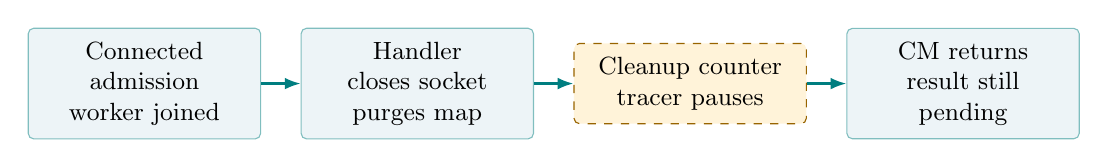
\begin{tikzpicture}[node distance=5mm and 5mm]
\node[box,text width=26mm] (admit) {Connected admission\\worker joined};
\node[box,text width=26mm,right=of admit] (purge) {Handler closes socket\\purges map};
\node[pending,text width=26mm,right=of purge] (trace) {Cleanup counter tracer pauses};
\node[box,text width=26mm,right=of trace] (cm) {CM returns\\result still pending};
\draw[arrow](admit)--(purge);\draw[arrow](purge)--(trace);\draw[arrow](trace)--(cm);
\end{tikzpicture}
\par\vspace{4mm}
\begin{itemize}\setlength\itemsep{2.5mm}
\item \textbf{Direct CM:} the handler result is still pending after CM returns. The unpaused control has a result at return.
\item \textbf{Pristine Server:} the scope has already finished when the test polls it with the tracer gate closed.
\item The Server test then opens the gate before it samples the handler result.
\end{itemize}
\evidence{SourceReplay, direct-CM self-purge (increments 78 and 99) and pristine full-Server control (increment 100). Both use synthetic inputs and a gated tracer.}
\end{frame}

\begin{frame}{Owned callers prove the original c2 statement}
\begin{block}{Variant policy}
\texttt{OwnedCallers} refuses foreign raw \texttt{beginAcquire}/\texttt{beginRelease}, including complete-plan aliases.
\end{block}\begin{itemize}\setlength\itemsep{2.5mm}
\item It guards the existing transitions and retains the original plan selection.
\item Restriction theorems map every variant run back to a source-model run.
\item At finished relays, initialized variant runs have no acquire or release frames.
\end{itemize}\small This is a caller ownership contract. It does not add a shutdown flag to pinned Haskell.
\evidence{Supervision increment 77; Variants/OwnedCallers; Properties/OwnedCallers, Protocols.no-frames; DesignContract, section 2.}
\end{frame}

\begin{frame}{Cancel-and-join admission workers loses a child}
\begin{itemize}\setlength\itemsep{2.5mm}
\item An include body is explicitly unmasked.
\item Cancellation can arrive after handler fork but before map publication.
\item Saved-map restoration restores the binding table while the physical child remains.
\item Joining the admission worker therefore leaves a handler outside the restored map.
\end{itemize}\begin{alertblock}{Rejected design}
The phase-A async probe and its post-publication control support this primitive window. They are not a CM/Server implementation replay or a maintained variant theorem.
\end{alertblock}
\evidence{Supervision increment 78, phase A; DesignContract, section 4; PrimitiveIncludeRestoration and HeapRollback.}
\end{frame}

\begin{frame}{Owning and joining workers is still insufficient}
\begin{block}{Phase B: own + join, without cancellation}
Worker joins prevent late admission and transport the original SI5 certificate.
\end{block}\begin{itemize}\setlength\itemsep{2.5mm}
\item Failed-handshake counterexample: the worker deletes its binding and joins while the handler remains in catch.
\item Successful-admission counterexample: the handler self-purges and remains pending after worker join.
\item Joining a handler only on failure/query still misses successful self-purge and other detachments.
\end{itemize}
\evidence{Supervision increment 78; Variants/ServerOwnedWorkers; Negative/ServerOwnedWorkersCounterexample and ServerOwnedWorkersSelfPurge.}
\end{frame}

\begin{frame}{Live-map membership cannot represent all births}
\small\renewcommand{\arraystretch}{1.2}
\begin{tabularx}{\textwidth}{@{}P{28mm}Y@{}}
\toprule
Detachment family & Historical handler that a live-map snapshot can miss \\ \midrule
Delete / self-purge & Inbound/outbound failure or query deletion; ordinary cleanup and TIME\_WAIT final purge. \\[2mm]
Aliases / publication & Outbound bracket alias cleanup; reservation/fork before publication; exception restoration. \\[2mm]
Overwrite / pruning & Same-entry overwrite, fresh replacement and Terminated pruning before physical completion. \\[2mm]
\bottomrule
\end{tabularx}\par\vspace{3mm}\small These are audited source routes. Collision reachability and some rollback windows retain separate scope obligations.
\evidence{Supervision increment 78, phase C; DesignContract, sections 4--5. Full per-route prototype replay remains an acceptance task.}
\end{frame}

\begin{frame}{Agda design for admission and handler ownership}
\centering
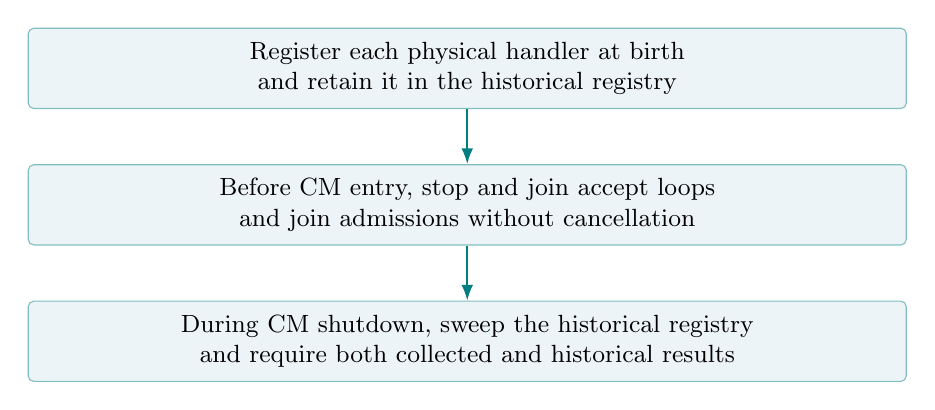
\begin{tikzpicture}[node distance=7mm]
\node[box,text width=108mm] (worker) {Register each physical handler at birth\\and retain it in the historical registry};
\node[box,text width=108mm,below=of worker] (history) {Before CM entry, stop and join accept loops\\and join admissions without cancellation};
\node[box,text width=108mm,below=of history] (sweep) {During CM shutdown, sweep the historical registry\\and require both collected and historical results};
\draw[arrow](worker)--(history);\draw[arrow](history)--(sweep);
\end{tikzpicture}
\par\vspace{3mm}\small Owned callers prevent new foreign CM work. The history survives deletion, overwrite, pruning and map restoration.

\evidence{Variants/ServerOwnedHandlers. Supervision increment 78. DesignContract, sections 1--2.}
\end{frame}

\begin{frame}{The registry design proves endpoint quiescence}
\begin{itemize}\setlength\itemsep{2.5mm}
\item \texttt{registry-si5}: original SI5 plus the completed registry sweep and results.
\item \texttt{no-late-admission}: at closingCM or serverReturned, raw workers are joined with results and cannot resume admission.
\item \texttt{quiescence}: at finished relays, every worker is joined and every registered/physical handler has a result.
\item \texttt{historical-quiescence}: earlier registered handlers also have endpoint results.
\end{itemize}\small Erasure relates variant steps to source-model steps, with registry bookkeeping stuttering and cancellation using existing delivery sites.
\evidence{Properties/ServerOwnedHandlers; DesignContract, section 2. Explicit initialize (O.initial core) profile. Safety conditional on reaching the endpoint.}
\end{frame}

\begin{frame}{Shutdown ordering in Agda and Haskell}
\small\renewcommand{\arraystretch}{1.2}
\begin{tabularx}{\textwidth}{@{}P{23mm}YY@{}}
\toprule
Boundary & Agda variant & Haskell prototype \\ \midrule
Admission joins & CM entry requires joined admissions and a joined IG. & Join inside the IG callback. A live IG can still consume notifications. \\[2mm]
Handler history & Sweep can interleave with map shutdown. CM closure requires all results. & Sweep starts when the map finalizer exits. Pending handlers are cancelled and joined concurrently. \\[2mm]
Caller scope & Variant guards foreign starts and late admission forks. & Scope ownership is a premise. An escaped handle can still include after return. \\[2mm]
\bottomrule
\end{tabularx}
\evidence{DesignContract, Model and prototype ordering. SourceReplay, increment 100. A correspondence proof for these orderings remains open.}
\end{frame}

\begin{frame}{CM-I4c reference validity is complete}
\begin{block}{Initialized theorem}
From \texttt{initialize (O.initial core) settings} and any \texttt{Runs} history, derive \texttt{FullValidity} without an extra invariant or history premise.
\end{block}\begin{itemize}\setlength\itemsep{2.5mm}
\item Combines physical resources, exact captures, phases, cleanup and negotiated chains.
\item Adds publication/failure snapshots, pool content, controls, PCs, tickets, jobs and saved-call owner/mux agreement.
\item The unrestricted initializer remains refuted by its preloaded-continuation counterexample.
\end{itemize}\small Recorded round-six acceptance: 18 fresh endpoint checks, with dependency interfaces reused and no warnings.
\evidence{Supervision increment 79, round six (12 November); Properties/LiveTrackerInitialized, from-initial; Negative/LiveTrackerInitialized. Separate from progress/source refinement.}
\end{frame}

\begin{frame}{G0--G5 are met within their declared scopes}
\small\renewcommand{\arraystretch}{1.2}
\begin{tabularx}{\textwidth}{@{}P{28mm}Y@{}}
\toprule
Gate & Accepted scope \\ \midrule
G0: domain/source & Reviewed finite LocalLifecycle profile and selected source inputs. \\[2mm]
G1: primitives & Selected primitive and dependency contracts with paired controls. \\[2mm]
G2: lifecycle & Finite inbound/outbound, failure, reuse, hot demotion and timeout paths. \\[2mm]
G3: concurrency & Initialized finite multi-peer and overlapping-incarnation histories. \\[2mm]
G4: semantics & Full raw supervised rendering, results, stable refusals and typed decoder. \\[2mm]
G5: exploration & Declared finite alphabets, checked exports/shrinking and classified replays. \\[2mm]
\bottomrule
\end{tabularx}
\evidence{GateAudit, 17 November. Whole-source refinement and universal progress remain open.}
\end{frame}

\begin{frame}{G1: the primitive matrix closed five runtime gaps}
\begin{itemize}\setlength\itemsep{2.5mm}
\item All selected primitive rows now have implemented rules and paired enabled/refusal controls.
\item Corrections cover configured-startup cancellation and include-body saved-map restoration.
\item Token grant refresh, handshake continuation outcomes and admission-fork failure now have distinct transitions.
\item Dependency evidence distinguishes IO from IOSim, including mask/delivery and waitCatch behavior.
\end{itemize}\small Timer expiry, elapsed time and blocking are supplied observations. Coverage does not establish a deadline or runtime equivalence.
\evidence{PrimitiveMatrix; Supervision increment 80; GateAudit G1. Capped regressions recorded as accepted, without weakening existing theorem statements.}
\end{frame}

\begin{frame}{G2: inbound release now has a physical receipt}
\begin{block}{The missing link}
Inbound release uses its actual captured target and masked send. Receipt interrupts the handler at explicitly unmasked TIME\_WAIT.
\end{block}\begin{itemize}\setlength\itemsep{2.5mm}
\item Normal responder/mux exit leads through physical release, socket/entry cleanup and IG unregistration.
\item Handler Async publication waits for the actual protected finally.
\item The clean body/mux path ends with an asynchronous handler result from TIME\_WAIT interruption.
\end{itemize}\small Cancellation receipt, caller return, completed cleanup and Async result availability remain separate transitions.
\evidence{Supervision increments 81--82; Negative/InboundCleanLifecycle; PrimitiveMatrix inbound receipt extension. Reduced finite profile, later extended to full responders.}
\end{frame}

\begin{frame}{G2: clean outbound and handshake failure are initialized}
\begin{itemize}\setlength\itemsep{2.5mm}
\item Clean outbound: establishment, activation, deactivation and close execute through real CM calls, mux/pool exit, release and Cold.
\item Handshake failure: observed deadline failure publishes the promise, returns Disconnected and runs real cleanup/result paths.
\item Endpoint and premature-step controls keep sockets, entries, captured handlers, jobs and monitors distinct.
\end{itemize}\begin{alertblock}{Witness scope}
These are enabled finite paths from the supervised initializer under supplied outcomes. The original clean path uses a reduced protocol bundle.
\end{alertblock}
\evidence{Supervision increment 83; Negative/OutboundCleanLifecycle and SupervisedHandshakeFailure. Full configured clean outbound follows in increment 92.}
\end{frame}

\begin{frame}{G2: production timeout cooling needs no foreign release}
\centering
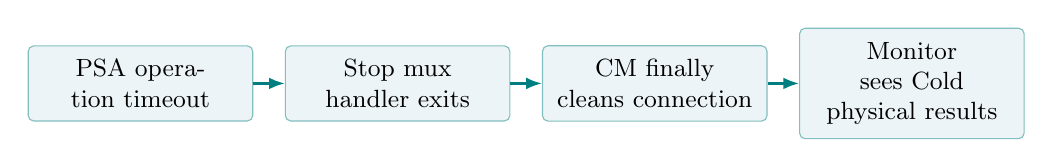
\begin{tikzpicture}[node distance=5mm and 4mm]
\node[box,text width=25mm] (timeout) {PSA operation timeout};
\node[box,text width=25mm,right=of timeout] (mux) {Stop mux\\handler exits};
\node[box,text width=25mm,right=of mux] (clean) {CM finally\\cleans connection};
\node[box,text width=25mm,right=of clean] (cold) {Monitor sees Cold\\physical results};
\draw[arrow](timeout)--(mux);\draw[arrow](mux)--(clean);\draw[arrow](clean)--(cold);
\end{tikzpicture}
\par\vspace{4mm}
\begin{itemize}\setlength\itemsep{2.5mm}
\item The complete initialized schedule executes under OwnedCallers.
\item No raw begin, invented CM release or TIME\_WAIT is needed on this route.
\item The separate foreign-caller TIME\_WAIT history remains a different example.
\end{itemize}
\evidence{Supervision increment 84, production-only witness; Negative/TimeoutCoolingOwned and TimeoutCoolingOwnedCallers. Supplied timeout observation, no elapsed-time theorem.}
\end{frame}

\begin{frame}{G3: real multi-peer and overlap histories}
\begin{block}{Two ordinary peers}
Both acquire, negotiate, execute protocol work, release and reach Cold with physical handler/job/monitor results. Their work and cleanup interleave.
\end{block}\begin{block}{Three same-key incarnations, plus another key}
Two old TIME\_WAIT finalizers are deferred until the third incarnation is live. Their eventual cleanup preserves the new and unrelated map entries.
\end{block}\small Both whole schedules execute under OwnedCallers. The overlap endpoint intentionally retains live handlers, so it is not a shutdown witness.
\evidence{Supervision increment 85; Negative/ConcurrentLifecycles and OverlapInitialized, facts and OwnedCallers certificates. Reduced finite profiles, selected interleavings.}
\end{frame}

\begin{frame}{G4: one machine now has a full raw CSP bridge}
\begin{itemize}\setlength\itemsep{1.8mm}
\item Inner and outer renderers use the actual supervised dispatcher, with exact successor states.
\item Step, finite-run and arbitrary-trace correspondence cover the complete typed raw runtime.
\item A lossless trace records before-state, action and after-state, retaining result observations.
\item An initialized lifecycle yields genuine CSP traces and a monitor-accepted run.
\end{itemize}\begin{alertblock}{Semantic boundary}
This is a rendering theorem. It does not establish independently composed parallel CSP, a compact API-only hiding abstraction or Haskell refinement.
\end{alertblock}
\evidence{Supervision increment 86; CSP/Supervised, SupervisedInner, Dispatcher, ResultTrace, RuntimeMonitor and SupervisedWitness.}
\end{frame}

\begin{frame}{G4: refusals and decoder coverage are exact}
\begin{itemize}\setlength\itemsep{2.5mm}
\item An arbitrary stable refusal set corresponds exactly to disabled machine actions at that state.
\item Stable failures correspond to actual runs ending in those disabled sets.
\item Visible raw labels and complete typed actions have unique encoding/decoding, including disabled actions and nested payloads.
\item The monitor connects replay refusals with rendered refusals in both directions.
\end{itemize}\small Tick is always refused and has no machine action. A typed decoder is separate from an external byte/log parser or source-operation coverage.
\evidence{Supervision increment 87; CSP/Dispatcher and SupervisedControls; GateAudit G4. Arbitrary states/full raw alphabet, no finite-carrier premise.}
\end{frame}

\begin{frame}{G0: branch review and protocol contracts}
\begin{itemize}\setlength\itemsep{2.5mm}
\item The branch matrix classifies implementation, contracted operations and explicit exclusions, with no missing rows.
\item ChainSync/BlockFetch contracts capture registry rendezvous, control sites, reply draining and cleanup.
\item TxSubmission2/KeepAlive contracts retain V2 choice, dq/dying state and finalizer dependencies.
\item Leios Notify/Fetch and shared resources retain control-read and cleanup order across the configured batch.
\end{itemize}\small Contracts record successful source-operation observations. Payloads, codecs, DB readiness and eventual reply/drain remain outside the lifecycle proof.
\evidence{BranchMatrix; ProtocolContracts; Supervision increments 88--90. Reviewed contracts are not native implementations of those protocols.}
\end{frame}

\begin{frame}{StartOnDemandAny resolved the configured-bundle blocker}
\begin{itemize}\setlength\itemsep{2.5mm}
\item Initiators start eagerly as in peer-state actions. Responders retain descriptor start modes.
\item Ordinary demand starts its waiter followed by the Any group; Any demand starts that group alone.
\item Any keys follow source map order, with separate trace/status/fork/registration steps.
\item Commands and results retain priority. Blocking tracers or cancellation can prevent later group members from starting.
\end{itemize}\small Paired controls cover ordering, duplicates, premature starts and interruption. Group selection does not imply an atomic group start or whole-group join.
\evidence{Supervision increments 91--92; Negative/StartOnDemandAny; BranchMatrix configured layout. Ingress payload queues remain abstract.}
\end{frame}

\begin{frame}{G2: full configured bundles now execute both ways}
\small\renewcommand{\arraystretch}{1.2}
\begin{tabularx}{\textwidth}{@{}P{28mm}Y@{}}
\toprule
Profile & Initialized, contract-coupled lifecycle \\ \midrule
Configured bundle & Hot: ChainSync, BlockFetch, TxSubmission2, LeiosNotify, LeiosFetch. Established: KeepAlive. Warm: empty. \\[2mm]
Outbound & All six initiators finish normal contracts, followed by clean demotion/close, physical results, release and Cold. \\[2mm]
Inbound & All six responders, including demand-triggered Any KeepAlive, finish contracts before mux exit, cleanup and IG unregistration. \\[2mm]
\bottomrule
\end{tabularx}\par\vspace{2mm}\small Immutable physical captures gate normal returns. Responders use a separate wrapper without outbound PSA control premises.
\evidence{Supervision increments 92 and 94; ConfiguredProtocols/ConfiguredResponders; FullConfiguredWitness/InboundConfiguredWitness. Normal bodies do not imply normal handler Async results.}
\end{frame}

\begin{frame}{G0/G2: source instantiation closes the selected profile}
\begin{itemize}\setlength\itemsep{2.5mm}
\item Selected V15/version data, flows and independent Tx V2 caller input are checked.
\item Full inbound/outbound runs use source policy constants: five retries and a 120-second failure-clear setting.
\item At the reached all-of-two and singleton decisions, picks are independent of seed/ranking for every finite commit/rollback/restart history.
\item Diffusion splits and the independent policy seed stay distinct; empty CM-bucket acquisition retains the source generator update.
\end{itemize}\small Topology, ready alternatives, clocks/order and operation outcomes are fixed. Other random readers, distributions and infinite retries remain outside the theorem.
\evidence{Supervision increments 93--96; SourceInputs/Negotiation, PolicyHistory, DiffusionSeeds, SeededConfigured and SourcePolicyInbound. Old reduced60 fixtures remain separately valid.}
\end{frame}

\begin{frame}{G5: bounded enumeration has explicit completeness}
\begin{itemize}\setlength\itemsep{2.5mm}
\item Enumerate all enabled dispatcher edges over a declared finite event list, through a finite depth and allocation cutoff.
\item Soundness yields real runs. Completeness includes every covered run within those bounds.
\item Six initialized G2/G3 witnesses have proved search membership.
\item Small relays controls compute searches. The six large search trees are not materialized.
\end{itemize}\begin{alertblock}{The alphabet is an explicit input}
Small ID ranges do not generate every constructor/payload combination. Exhaustion means no enabled event in the declared alphabet, not global deadlock.
\end{alertblock}
\evidence{Exploration/README stage 1; Supervision increment 97; Exploration/Bounded, Supervised and witness modules.}
\end{frame}

\begin{frame}{G5: checked exports and targeted race searches}
\begin{itemize}\setlength\itemsep{2.5mm}
\item Dictionary-relative text round trips through the parser and actual dispatcher, retaining full typed actions.
\item Six exported initialized traces are byte-verified and re-imported with exact endpoint certificates.
\item Late-admission and self-purge searches use reached local windows; the foreign-frame search starts from initialization.
\item Known source-model candidates have proved membership. Registry/ownership variants have bounded negative results.
\end{itemize}\small Membership proofs differ from executed exhaustive searches. The combined late-registry filtered negative also computes its search result.
\evidence{Exploration/README stage 2; Supervision increment 98. Exact dictionaries/windows/bounds in appendix. No general Haskell log format or new replay claim.}
\end{frame}

\begin{frame}{G5: shrinking preserves initialization and the violation}
\small\renewcommand{\arraystretch}{1.2}
\begin{tabularx}{\textwidth}{@{}P{28mm}Y@{}}
\toprule
Candidate & Checked original to reduced schedule \\ \midrule
Late admission & \textbf{50 to 46 events}: returned Server, closed empty CM snapshot and physical child present. \\[2mm]
Self-purge & \textbf{85 to 82 events}: finished relays, closed CM and a physical handler without its result. \\[2mm]
Foreign frame & \textbf{192 to 183 events}: finished relays with the external acquisition frame retained. \\[2mm]
\bottomrule
\end{tabularx}\par\vspace{2mm}\small External deletion proposals are independently checked by literal Agda certificates. Same initializer, dictionary payloads and violation predicate. No global-minimum theorem.
\evidence{Supervision increment 99; Exploration/Minimise, MinimiseCandidates and ShrunkLate/Purge/Foreign. Original and reduced text artifacts retained.}
\end{frame}

\begin{frame}{G5: reduced source tests retain three classifications}
\small\renewcommand{\arraystretch}{1.2}
\begin{tabularx}{\textwidth}{@{}P{28mm}Y@{}}
\toprule
Candidate & Pinned IOSim observation and control \\ \midrule
Late admission & Harness include after CM return succeeds. Combined race with the original Server worker remains unconfirmed. \\[2mm]
Self-purge & Handler result stays pending across CM return at the gated cleanup tracer. Immediate-tracer control has a result. \\[2mm]
Foreign caller & Externally forked caller survives CM return. Joining it first removes the residue: ownership over-approximation. \\[2mm]
\bottomrule
\end{tabularx}\par\vspace{3mm}\textbf{Recorded result:} all five tests passed after an offline serial build. These replay selected operations, not imported Agda schedules.
\evidence{SourceReplay, reduced cleanup candidates; Supervision increment 99. Synthetic sockets/handshake, explicit watchdogs and completed harness joins. No exhaustive schedule search.}
\end{frame}

\begin{frame}{Pinned Haskell prototype results}
\small\renewcommand{\arraystretch}{1.2}
\begin{tabularx}{\textwidth}{@{}P{31mm}Y@{}}
\toprule
Recorded check & Result \\ \midrule
Pristine source & 11 original defect/control checks reproduced. Four positive quiescence assertions failed. \\[2mm]
Patched source & 18 IOSim checks passed, including five teardown routes, Server self-purge and pre-publication rollback. Four checks deliberately expose blocked progress. \\[2mm]
Bounded schedules & Two prototype POR properties explored 597 schedules each at bounds 20,000/20. \\[2mm]
Existing suite & 37 properties passed at 100 cases. IG-race timed out at 100 on both versions and passed at 10. \\[2mm]
\bottomrule
\end{tabularx}
\evidence{SourceReplay and Supervision, increment 100. Fixtures and finite schedules constrain each observation.}
\end{frame}

\begin{frame}{Open shutdown obligations}
\begin{itemize}\setlength\itemsep{2.5mm}
\item Guarantee terminal handshake publication or define recovery for an empty promise.
\item Define how admission notifications finish after IG exits, when the bounded queue has no consumer.
\item Establish cleanup and callback progress and reconcile the Haskell join/sweep ordering with Agda.
\item Extend physical-result coverage to the remaining detachments and listener configurations.
\end{itemize}
\begin{alertblock}{Pristine source investigation}
The delayed Server worker and post-return direct include have been observed separately. Confirmation of the combined race requires a single source trace.
\end{alertblock}
\evidence{DesignContract, sections 3--5 and ordering comparison. GateAudit, second objective. SourceReplay, increment 100.}
\end{frame}

\appendix

\begin{frame}{Appendix: source authority and evidence map}
\small
\textbf{Network}\par
\texttt{2f1c154f248659b89523d5679ca532f442e7ed2a}\par\vspace{2mm}
\textbf{Consensus}\par
\texttt{2e44d98a843168ba3b189e305820b79943ac7d1e}\par\vspace{3mm}
\begin{itemize}\setlength\itemsep{2.5mm}
\item Supervision: dated increments and recorded check outcomes.
\item GateAudit: current acceptance scope, superseding historical open statements.
\item BranchMatrix / PrimitiveMatrix / ProtocolContracts: source and contract boundaries.
\item CM\_Summary and November architecture review: findings, proof scope and prototype differences.
\end{itemize}
\evidence{SourceLedger and GateAudit. November architecture review, section 11.}
\end{frame}

\begin{frame}{Appendix: shutdown and residue proof endpoints}
\small\renewcommand{\arraystretch}{1.2}
\begin{tabularx}{\textwidth}{@{}P{28mm}Y@{}}
\toprule
Claim & Maintained evidence under Properties/ \\ \midrule
SI5a / SI5b & \texttt{ServerShutdownComplete} / \texttt{ServerShutdownCoordinator} \\[2mm]
IG residue c1 & \texttt{IGPendingQuiet.Protocols.ig-quiet} \\[2mm]
Foreign-only c2 & \texttt{ForeignFrames.Protocols.foreign-frames} \\[2mm]
Owned-callers c2 & \texttt{OwnedCallers.Protocols.no-frames} \\[2mm]
Registry quiescence & \texttt{ServerOwnedHandlers}: registry-si5, no-late-admission, quiescence, historical-quiescence \\[2mm]
\bottomrule
\end{tabularx}
\evidence{Supervision increments 71--78; DesignContract, section 2. Initializers and runtime variants are part of each theorem's scope.}
\end{frame}

\begin{frame}{Appendix: configured profile and invariant scope}
\small\renewcommand{\arraystretch}{1.2}
\begin{tabularx}{\textwidth}{@{}P{28mm}Y@{}}
\toprule
Item & Exact boundary \\ \midrule
LocalLifecycle & One post-setup listener; two known ordinary peers; targets known/established/active = 2/2/1. \\[2mm]
Full configured runs & Outbound: 381 wrapper inputs / 322 frontend events. Inbound: 246 / 208. Explicit observed contracts. \\[2mm]
CM-I4c & \texttt{LiveTrackerInitialized.from-initial} derives FullValidity for \texttt{initialize (O.initial core) settings}. \\[2mm]
Excluded inference & No whole-node boot, unrestricted preloaded initializer, arbitrary source selection, payload correctness or universal shutdown claim. \\[2mm]
\bottomrule
\end{tabularx}
\evidence{BranchMatrix; ProtocolContracts; SourceInputs source-profile runs; Supervision increment 79 round six and increments 92--96.}
\end{frame}

\begin{frame}{Appendix: exact exploration windows and bounds}
\small\renewcommand{\arraystretch}{1.2}
\begin{tabularx}{\textwidth}{@{}P{28mm}Y@{}}
\toprule
Search & Declared scope \\ \midrule
Ordinary witnesses & Six initialized paths: handshake failure, inbound, timeout, outbound, two peers and same-key overlap. Proved membership. \\[2mm]
Late admission & Server-layer reached shutdown/admission window. Depth/capacity 10/8. Same-window worker and registry comparisons. \\[2mm]
Self-purge & Reached pre-close-to-finished window. Depth/physical-handler capacity 16/8, including repaired continuation labels. \\[2mm]
Foreign frame & Full initialized run, depth bound 1000. Exact finite alphabet, with allocation pruning disabled. \\[2mm]
\bottomrule
\end{tabularx}\par\vspace{2mm}\small Finite dictionaries retain concrete IDs and supplied outcomes. These scopes do not enumerate all small-ID payloads.
\evidence{Exploration/README stages 1--2; Supervision increments 97--98. Bounds are not witness lengths or global unreachability results.}
\end{frame}

\begin{frame}{Appendix: prototype progress failures}
\small\renewcommand{\arraystretch}{1.2}
\begin{tabularx}{\textwidth}{@{}P{28mm}Y@{}}
\toprule
Controlled failure & IOSim observation \\ \midrule
Blocked cleanup & A permanently closed cleanup-tracer gate prevents the physical result and blocks both CM and Server teardown. \\[2mm]
Empty promise & The handler finishes and purges its map entry. Server still waits for admission, before CM shutdown starts. \\[2mm]
IG queue pressure & After IG exits, 100 notifications commit. The 101st producer blocks admission and Server cannot begin CM shutdown. \\[2mm]
\bottomrule
\end{tabularx}\par\vspace{2mm}
The empty-promise and queue cases stall before the historical sweep can run.
\evidence{SourceReplay, increment 100, Progress findings and limits. DesignContract, section 3.}
\end{frame}

\begin{frame}[fragile]{Appendix: build the editable deck}
\small
From the library root:
\begin{lstlisting}
make -C ConnectionManagement/Presentations \
  SOURCE=progress-2026-11-17.tex check
\end{lstlisting}
PDF output:
\begin{lstlisting}
output/pdf/connection-management-progress-2026-11-17.pdf
\end{lstlisting}
\evidence{ConnectionManagement/Presentations/Makefile and README.}
\end{frame}

\end{document}
